\documentclass[]{beamer}
\usepackage{xmpmulti}
\usepackage{psfrag}
\usepackage{xcolor}
\usepackage{chessboard}
\newcommand{\owner}{\mathcal{O}}
\newcommand{\manager}{\mathcal{M}}

\usepackage{tikz}
\usetikzlibrary{snakes}
\usetikzlibrary{backgrounds} 
\usepackage{pgfmath}


\mode<presentation>
{\usetheme{Boadilla}  % very plain
}

\usepackage{xcolor}

\usepackage{amssymb,amsmath,amsthm}
\usepackage{boxedminipage}

\setbeamercolor{uppercol}{fg=teal,bg=lightgray}%
\setbeamercolor{lowercol}{fg=olive,bg=lightgray!50}%

\newcommand{\curr}{\mathtt{current}}
\newcommand{\mos}{\mathtt{m}}
\newcommand{\move}{\mathtt{lmove}}
\newcommand{\nmove}{\mathtt{nmove}}

\title[]{Symmetric Encryption with OpenSSL}

\author{Giuseppe Persiano}

\institute[UNISA]{%
Universit\`a di Salerno\\ \qquad \\
}

\date[November 2020]{November, 2020}

\begin{document}

{
\begin{frame}
  \titlepage
\end{frame}
\begin{frame}
\frametitle{Encrypting with OpenSSL}
\begin{block}{\tt openssl enc}
Parameters:
\begin{itemize}
\item {\tt -in}: input file
\item {\tt -out}: output file
\item specify the algorithm
\item specify the key
\end{itemize}
\end{block}
\end{frame}

\begin{frame}
\frametitle{Encrypting with AES}
\begin{block}{openssl enc: specifying the algorithm}
\begin{itemize}
\item{\tt AES, Blowfish, Camellia, Chacha20, SEED, CAST-128, DES, IDEA, RC5, Triple DES}

\item {\tt AES}:
    \begin{itemize}
        \item {\color{red} 128 bit keys:}

        {\tt AES-128-CBC, AES-128-CBC-HMAC-SHA1, 
             AES-128-CBC-HMAC-SHA256, 
             id-aes128-CCM, 
             id-aes128-GCM, 
             AES-128-CFB, 
             AES-128-CFB1, 
             AES-128-CFB8, 
             AES-128-CTR, 
             AES-128-ECB, 
             AES-128-OCB, 
             AES-128-OFB, 
             AES-128-XTS}

        \item {\color{red} 256-bit keys:}

        {\tt AES-256-CBC, AES-256-CBC-HMAC-SHA1, 
             AES-256-CBC-HMAC-SHA256, 
             id-aes256-CCM, 
             AES-256-CFB, 
             AES-256-CFB1, 
             AES-256-CFB8, 
             AES-256-CTR, 
             AES-256-ECB, 
             id-aes256-GCM, 
             AES-256-OCB, 
             AES-256-OFB, 
             AES-256-XTS}

\item {\color{red} shortcuts:}

        {\tt aes128 $\Rightarrow$ AES-128-CBC, 
             aes128-wrap $\Rightarrow$ id-aes128-wrap, 
             aes192 $\Rightarrow$ AES-192-CBC, 
             aes192-wrap $\Rightarrow$ id-aes192-wrap, 
             aes256 $\Rightarrow$ AES-256-CBC, 
             aes256-wrap $\Rightarrow$ id-aes256-wrap
        }
\end{itemize}
\end{itemize}
\end{block}
\end{frame}

\begin{frame}
\frametitle{Encrypting with AES}
\begin{block}{openssl enc: using a password}
\begin{itemize}
\item openssl derives a key from a {\em password} + {\em salt} 
using a key derivation function KDF
\item OpenSSL 1.1.1f, PBKDF1 (with $c=1$)  and SHA256
        \begin{itemize}
            \item {\tt KEY=SHA256(Password||Salt)}
            \item {\tt IV=SHA256(KEY||Password||Salt)}
        \end{itemize}
\end{itemize}
\end{block}

\begin{center}
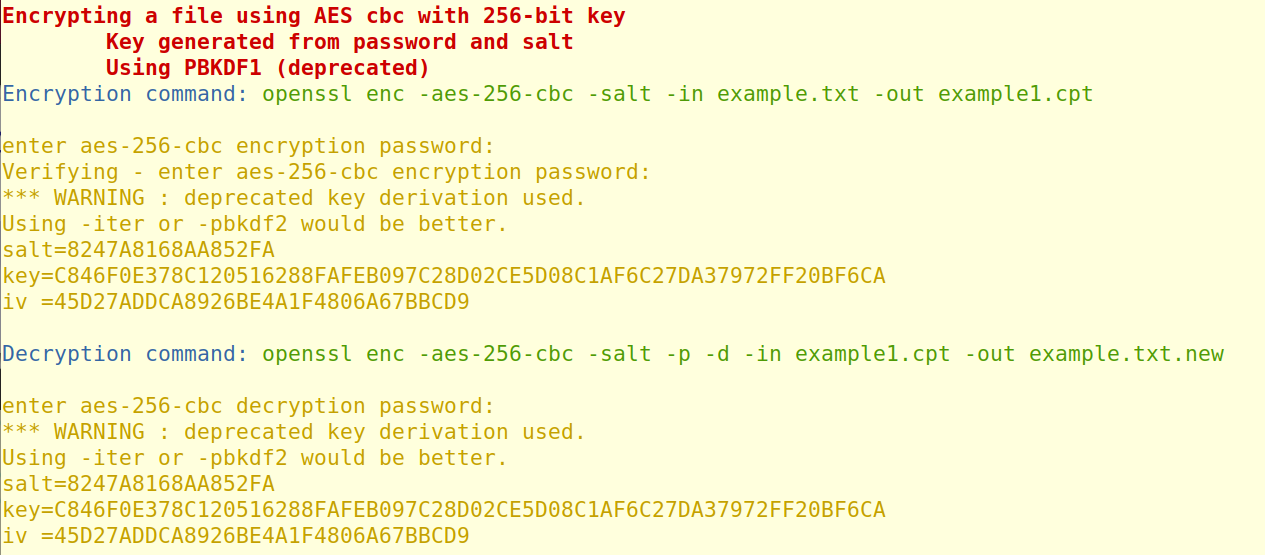
\includegraphics[width=3.6in]{imgs/PBKDF1.png}
\end{center}
\end{frame}

\begin{frame}
\frametitle{Encrypting with AES}
\begin{block}{openssl enc: using a password}
\begin{itemize}
\item We can specify {\tt -pbkdf2} or {\tt -iter} followed by the number
of iterations that will force the use of PBKDF2
\end{itemize}
\end{block}
\begin{center}
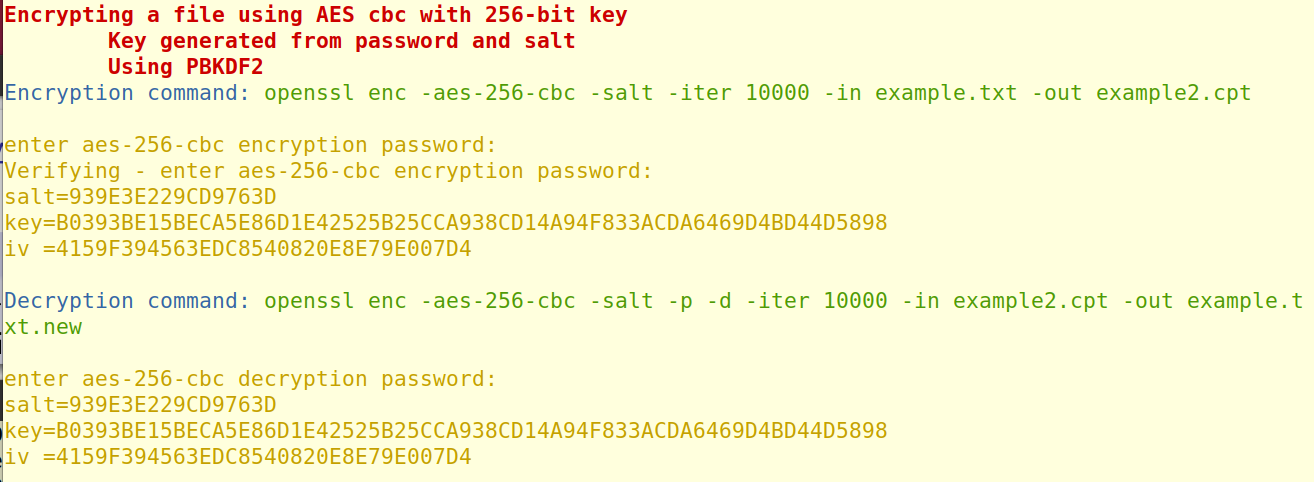
\includegraphics[width=4in]{imgs/PBKDF2.png}
\end{center}
\end{frame}

\begin{frame}
\frametitle{Salted File Format}
\begin{center}
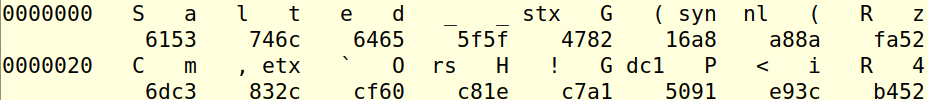
\includegraphics[width=4in]{imgs/saltedFile.png}
\end{center}
\end{frame}

\begin{frame}
\frametitle{PBKDF1}
\begin{itemize}
\item uses a {\sf Hash} function (SHA-256, by default)
\item {\color{blue} inputs}:
    \begin{itemize}
        \item $P$: password
        \item $S$: salt, 8-byte string
        \item $c$: iteration count $\geq 1$
        \item $\tt{dkLen}$: length of the derived key
    \end{itemize}
\item {\color{blue} algorithm}:
    \begin{itemize}
    \item $T_1=\mathsf{Hash}(P||S)$
    \item $T_2=\mathsf{Hash}(T_1)$
    \item $\ldots\ldots$
    \item $T_c=\mathsf{Hash}(T_{c-1})$
    \item Output first $\tt{dkLen}$ byte of $T_c$
\end{itemize}
\end{itemize}
{\tt openssl} uses $c=1$ with SHA-256 as a default
\end{frame}

\begin{frame}
\frametitle{PBKDF2}
\begin{itemize}
\item $\color{red}\mathtt{DK = PBKDF2(PRF, Password, Salt, c, dkLen)}$
\item $\color{red}\mathtt{DK = T1|| T2 ||\ldots ||Tdklen/hlen}$
    \begin{itemize}
       \item $\mathtt{Ti = F(Password, Salt, c, i)}$
       \item $\mathtt{F(Password,Salt,c,i)=U_1\oplus U_2\oplus\cdots\oplus U_c}$
       \item $\mathtt{U_1=PRF(Password, Salt||i)}$
       \item $\mathtt{U_2=PRF(Password, U_1)}$
       \item $\ldots\ldots$
       \item $\mathtt{U_c=PRF(Password, U_{c-1})}$
    \end{itemize}

\medskip

The PRF used is HMAC-SHA-256
\end{itemize}
\end{frame}

\begin{frame}
\frametitle{Encrypting with AES}
\begin{block}{openssl enc: specifying a password and the IV}
\begin{itemize}
\item use {\tt -K} followed by the key in hexadecimal
\item use {\tt -iv} followed by the IV in hexadecimal
\end{itemize}
\end{block}

\vskip 2cm

\begin{center}
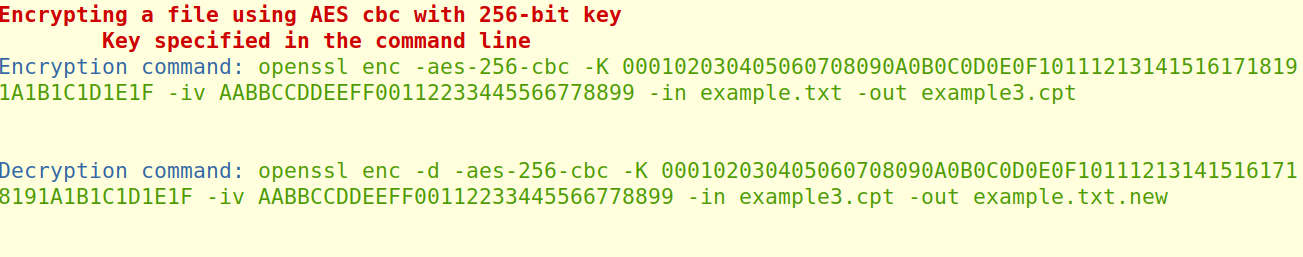
\includegraphics[width=4in]{imgs/encwithKey.png}
\end{center}

\end{frame}

\begin{frame}
\frametitle{Encrypting with AES}
\begin{block}{openssl enc: randomly generating a password and the IV}
\begin{itemize}
\item use command {\tt openssl rand -hex 32}  to generate the 32 bytes
    needed for an AES-256 key
\item use command {\tt openssl rand -hex 16}  to generate the 16 bytes
    needed for an AES-256 IV
\end{itemize}

\end{block}
\end{frame}
\end{document}
